%!TEX root = main.tex

\section{Prioritized Streaming String Transducers}  \label{sect:psst}
%\zhilin{Move from preliminary to here}

In this section, we introduce prioritized streaming string transducers (PSST), which extends prioritized finite-state automata (PFA) proposed in \cite{BM17}. We shall utilize PSST to model  the eager and greedy semantics of $\regexp$ as well as the behavior of $\replaceall$ functions where both capturing groups and back references occur.
%based on which we model the semantics of $\regexp$ defined in Section~\ref{sec:prel} and design the decision procedure in Section~\ref{sec:decision}.

%\paragraph{Prioritized Finite-state automata.}
%
For a finite set $Q$, let $\overline{Q} = \bigcup_{n\in \Nat}\{ (q_1, \ldots, q_n) \mid \forall i \in [n], q_i \in Q \wedge \forall i,j \in[n], i \neq j \rightarrow q_i \neq q_j \}$. Intuitively, $\overline{Q}$ is the set of sequences of non-repetitive elements from $Q$. In particular, the empty sequence $\varepsilon \in \overline{Q}$. Note that the length of each sequence from $\overline{Q}$ is bounded by  $| Q |$. For a sequence $P = (q_1, \ldots, q_n) \in \overline{Q}$ and  $q \in Q$, we write $q \in P$ if  $q = q_i$ for some $i \in [n]$. Moreover, for $P_1 = (q_1, \ldots, q_m) \in \overline{Q}$ and $P_2 = (q'_1, \ldots, q'_n) \in \overline{Q}$, we say $P_1 \cap P_2 = \emptyset$ if $\{q_1, \ldots, q_m\} \cap \{q'_1, \ldots, q'_n\} = \emptyset$.


\begin{definition}[Prioritized Finite-state Automata]\label{def-pfa}
  A \emph{prioritized finite-state automaton} (PFA) over a finite alphabet $\Sigma$ is a tuple $\pnfa=(Q, \Sigma, \delta, \tau, q_0, F)$ where $\delta \in Q
  \times \Sigma \rightarrow \overline{Q}$ and $\tau \in Q \rightarrow \overline{Q} \times \overline{Q}$ such that for every $q \in Q$, if $\tau(q) = (P_1; P_2)$, then $P_1 \cap P_2 = \emptyset$. 
  The definition of $Q$, $q_0$ and $F$ is the same as ordinary FA.
\end{definition}
For $\tau(q) = (P_1; P_2)$, we will use $\pi_1(\tau(q))$ and $\pi_2(\tau(q))$ to denote $P_1$ and $P_2$ respectively.  With slight abuse of notation, we write $q\in (P_1; P_2)$ for $q\in P_1\cup P_2$. Intuitively, $\tau(q)=(P_1; P_2)$ specifies the $\varepsilon$-transitions at $q$, with the intention that the $\varepsilon$-transitions to the states in $P_1$ resp. $P_2$ have higher resp. lower priorities than the non-$\varepsilon$-transitions out of $q$.
  
A  run of $\pnfa$ on a string $w$ is a sequence $q_0 \sigma'_1 q_1 \ldots \sigma'_m q_m$ such that 
\begin{itemize}
%\item $q_m \in F$,
\item for any $i \in [m]$, either $\sigma'_i \in \Sigma$ and $q_i \in \delta (q_{i - 1}, \sigma'_i)$, or $\sigma'_i = \varepsilon$ and $q_i \in \tau(q_{i-1)}$ %\pi_1(\tau(q_{i-1}))\cup \pi_2(\tau(q_{i-1}))$,
\item $w = \sigma'_1 \cdots \sigma'_m$,
%
\item for every subsequence $q_i \sigma'_{i+1} q_{i+1} \ldots \sigma'_{j} q_j$ such that  $i < j$ and $\sigma'_{i+1} = \cdots = \sigma'_j = \varepsilon$, it holds that $q_i, \ldots, q_j$ are mutually distinct. (Intuitively, loops of $\varepsilon$-transitions are forbidden.) 
\end{itemize}
Note that it is possible that $\delta(q, \sigma) = ()$, namely, there is no $\sigma$-transition out of $q$. 
It is easy to observe that given a string $w$, the length of a run of $\pnfa$ on $w$ is $O(|w||Q|)$.
For any two runs $p = q_0 \sigma_1 q_1 \ldots \sigma_m q_m$ and $p' =  q_0 \sigma'_1 q_1' \ldots \sigma'_n q'_n$ such that $\sigma_1 \ldots \sigma_m = \sigma'_1 \ldots \sigma'_n$, we say that $p$ is of a higher priority over $p'$ if 
\begin{itemize}
\item either $p'$ is a prefix of $p$ (in this case, the transitions of $p$ after $p'$ are all $\varepsilon$-transitions), 
%
\item or there is an index $j$ satisfying one of the following constraints:
\begin{itemize}
\item $q_0 \sigma_1 q_1 \ldots q_{j-1} \sigma_j = q_0 \sigma'_1 q'_1 \ldots q'_{j-1} \sigma'_j$, $q_j \neq q'_j$, $\sigma_j \in \Sigma$, and $\delta (q_{j - 1}, \sigma_j) =(\ldots, q_j, \ldots, q_j', \ldots)$,
%
\item $q_0 \sigma_1 q_1 \ldots q_{j-1} \sigma_j = q_0 \sigma'_1 q'_1 \ldots q'_{j-1} \sigma'_j$, $q_j \neq q'_j$, $\sigma_j  = \varepsilon$,  and  either $\pi_1(\tau(q_{j - 1})) = (\ldots, q_j, \ldots, q_j', \ldots)$, or $\pi_2(\tau(q_{j - 1})) = (\ldots, q_j, \ldots, q_j', \ldots)$, or $q_j \in \pi_1(\tau(q_{j - 1}))$ and $q'_j \in \pi_2(\tau(q_{j-1}))$, 
%
\item $q_0 \sigma_1 q_1 \ldots q_{j-1}  = q_0 \sigma'_1 q'_1 \ldots q'_{j-1} $, $\sigma_j  = \varepsilon$, $\sigma'_j  \in \Sigma$, $q_j \in \pi_1(\tau(q_{j - 1}))$, and $q'_j \in \delta(q_{j-1}, \sigma'_j)$, 
%
\item $q_0 \sigma_1 q_1 \ldots q_{j-1}  = q_0 \sigma'_1 q'_1 \ldots q'_{j-1} $, $\sigma_j  \in \Sigma$, $\sigma'_j  = \varepsilon$, $q_j \in \delta(q_{j - 1}, \sigma_j)$, and $q'_j \in \pi_2(\tau(q_{j-1}))$.
\end{itemize}
\end{itemize}

The \emph{accepting} run of $\pnfa$ on $w$ is a run $q_0 \sigma_1 q_1 \ldots \sigma_m q_m$ of $\pnfa$ on $w$ with the \emph{highest} priority such that $q_m \in F$. The language of $\pnfa$, denoted as $\Lang(\pnfa)$, is the set of
 strings on which $\pnfa$ has an accepting run.


Note that PFAs differ from FAs only in the way that the strings are accepted, they still define regular languages. 

\begin{example}
The PFAs corresponding to $a^\ast$ and $a^{\ast?}$ respectively are illustrated in Figure~\ref{fig-pfa}: (i) and (ii), where the dashed line represents $\pi_2(\tau(q_0))$ (of lower priority than the $a$-transition), the thicker solid line represents $\pi_1(\tau(q_0))$ (of higher priority than the $a$-transition), and the doubly circled state $q_1$ is a final state.

\begin{figure}[ht]
\centering
%\rule{\linewidth}{0cm}
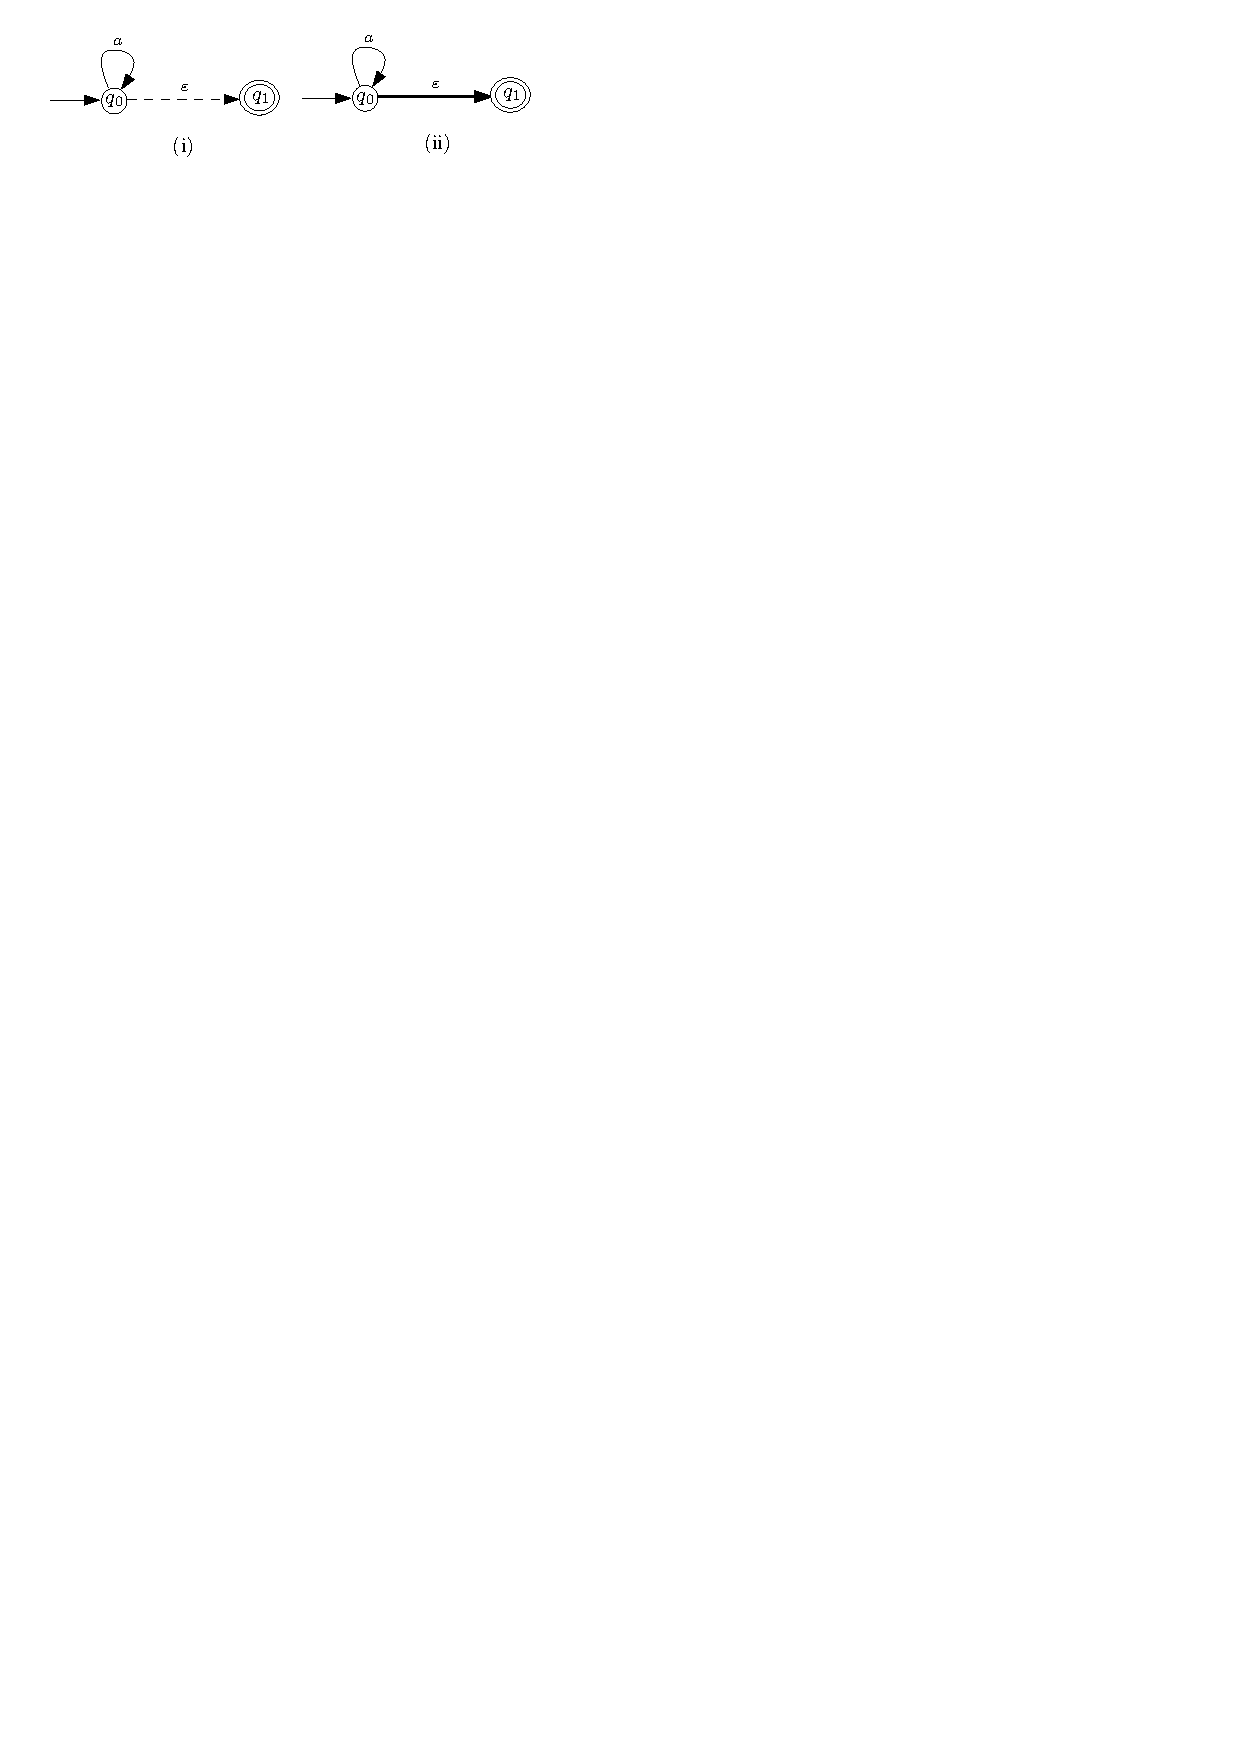
\includegraphics[scale=0.8]{pfa.pdf}
\caption{The PFAs for $a^\ast$ and $a^{\ast?}$}
\label{fig-pfa}
\end{figure}

\end{example}

\begin{remark}
Remark that PFAs in Definition~\ref{def-pfa} are different from pNFAs in \cite{BM17} in the sense that the state set in a pNFA is partitioned into two disjoint subsets and the non-$\varepsilon$-transitions are deterministic, while this is not the case in PFAs. We choose this definition of PFAs as a more natural extension of FAs. 
\end{remark}

The priorities of PFAs are used to model the eager and greedy semantics of $\regexp$, as we shall see in Section~\ref{construction:pnfa}.


%\paragraph{Prioritized streaming string transducers.}

We then introduce prioritized streaming string transducers, a new class of transducers that combine prioritized transducers \cite{BM17} %which combines the expressive power of 
and streaming string transducers \cite{AC10,AD11}.
  
\begin{definition}[Prioritized Streaming String Transducers]
A \emph{prioritized streaming string transducer} (PSST) is a tuple $\psst = (Q, \Sigma, X, \delta, \tau, E, q_0, F)$, where $Q$ a
finite set of states, $\Sigma$ is the input and output alphabet, $X$ is a finite set of variables, $\delta \in Q \times \Sigma \rightarrow \overline{Q}$, $\tau \in Q \rightarrow \overline{Q} \times \overline{Q}$, $E$ is a partial function from $Q \times \Sigma^\varepsilon \times
  Q$ to $X \rightarrow (X \cup \Sigma)^{\ast}$, i.e. the set of assignments,
   $q_0 \in Q$ is the initial state, and $F$ is a partial function
  from $Q$ to $(X \cup \Sigma)^{\ast}$.

A run of $\psst$ on a string $w$ is a sequence $q_0 \sigma_1 s_1 q_1 \ldots \sigma_m s_m q_m$ such that
\begin{itemize}
%\item $q_m \in F$,
%
\item for each $i \in [m]$, 
\begin{itemize}
\item either $\sigma_i \in \Sigma$, $q_i \in \delta (q_{i-1}, \sigma_i)$, and $s_i = E (q_{i - 1}, \sigma_i, q_i)$, 
\item or $\sigma_i = \varepsilon$, $q_i \in \tau(q_{i-1})$ and $s_i = E (q_{i - 1}, \varepsilon, q_i)$.
\end{itemize}

\item for every subsequence $q_i \sigma_{i+1} s_{i+1} q_{i+1} \ldots \sigma_{j} s_j q_j$ such that  $i < j$ and $\sigma_{i+1} = \cdots = \sigma_j = \varepsilon$, it holds that $q_i, \ldots, q_j$ are mutually distinct. (Intuitively, loops of $\varepsilon$-transitions are forbidden.) 
\end{itemize}

%A run of $\psst$ is the sequence $q_0 \sigma_1 s_1 q_1 \ldots \sigma_m s_m q_m$, where $F (q_m)$ is defined and for each $i \in [m], q_i \in \delta (q_{i-1}, \sigma_i)$ and $s_i = E (q_{i - 1}, \sigma_i, q_i)$. 
For any pair of runs $p = q_0 \sigma_1 s_1 \ldots \sigma_m s_m q_m$ and $p' = q_0 \sigma'_1
  s_1' \ldots \sigma'_n s_n' q_n'$ such that $\sigma_1 \ldots \sigma_m = \sigma'_1 \ldots \sigma'_n$, the definition that $p$ is of a higher priority over
  $p'$ is similar to PFAs.
  % $p \neq p'$ and, for the smallest index $j$ with $q_j \neq q_j'$,
 % $\delta (q_{j - 1}, \sigma_j) = \ldots q_j \ldots q_j' \ldots$
  
The accepting run of $\psst$ on an input $w$ is a run of $\psst$ on $w$ of the highest priority, say $q_0 \sigma_1 s_1 \ldots \sigma_m s_m q_m$, such that $F(q_m)$ is defined. The output of $\psst$ on $w$, denoted by $\psst(w)$, is defined as $\eta_m(F(q_m))$, where $\eta_0(x) = \varepsilon$ for each $x \in X$, and $\eta_{i}(x) = \eta_{i-1}(s_{i}(x))$ for every $1 \le i \le m$ and $x \in X$. Note that here we abuse the notation  $\eta_m(F(q_m))$ and $\eta_{i-1}(s_{i}(x))$ by taking a function $\eta$ from $X$ to $\Sigma^*$ as a function from $(X \cup \Sigma)^*$ to $\Sigma^*$, which maps each $\sigma \in \Sigma$ to $\sigma$ and each $x \in X$ to $\eta(x)$. If there is no accepting run of $\psst$ on $w$, then $\psst(w) = \bot$, namely, the output of $\psst$ on $w$ is undefined. The string relation defined by $\psst$, denoted by $\cR_\psst$,  is $\{(w, \psst(w)) \mid w \in \Sigma^\ast, \psst(w) \neq \bot\}$.
\end{definition}

\begin{example}
The PSST $\cT_{\sf nameReg}=(Q, \Sigma, X, \delta, \tau, E,  q_{0}, F)$ mentioned in Section~\ref{sec:mot} is illustrated in Figure~\ref{fig-psst-exmp}, where $Q = \{q_0, \dots, q_{24}\}$, $X= \{x_1, x_2, x_3, x_4\}$ with $x_1, x_2, x_3$ recording the matches of the 1st, 2nd, 3rd capturing group, and $x_4$ recording the string after the replacements, $F(q_{24}) = x_4$ denotes the final output, and $\delta, \tau, E$ are illustrated by the edges, where the dashed edges denote the $\varepsilon$-transitions of lower priorities than the non-$\varepsilon$-transitions and the symbol $\ell$ is used to denote the currently scanned input letter. For instance, $\delta(q_3, \backslash\mbox{s}) = (q_3)$, $\delta(q_3, \ell) = ()$ for every $\ell \in \Sigma \setminus \{\backslash\mbox{s}\}$, $\tau(q_3) = ((); (q_4))$, and $E(q_3, \backslash\mbox{s}, q_3)(x_1) = x_1 \backslash s$. Since the $\varepsilon$-transition has lower priority than the $\backslash\mbox{s}$-transition at the state $q_3$, whenever the currently scanned letter is $\backslash$s at $q_3$,  $\cT_{\sf nameReg}$ will choose to go to $q_3$ greedily, until there is no more $\backslash$s. (In this case, it has to choose the $\epsilon$-transition and goes to $q_4$.) Note that the identity assignments, e.g. $E(q_3, \backslash\mbox{s}, q_3)(x') = x'$ for $x' \in \{x_2, x_3, x_4\}$, are omitted in Figure~\ref{fig-psst-exmp}, for readability. 
%From $\delta(q_4, \backslash s) = q_5q_{6}$, we know that $q_5$ is prior to $q_6$. 
%Therefore, whenever $\cT_{\sf nameReg}$ reads $\backslash$s at the state $q_3$,  it will choose to go the state $q_5$ greedily, unless this choice would lead to the nonacceptance (in this case, $q_6$ will be chosen). 
\begin{figure*}[ht]
\centering
%\rule{\linewidth}{0cm}
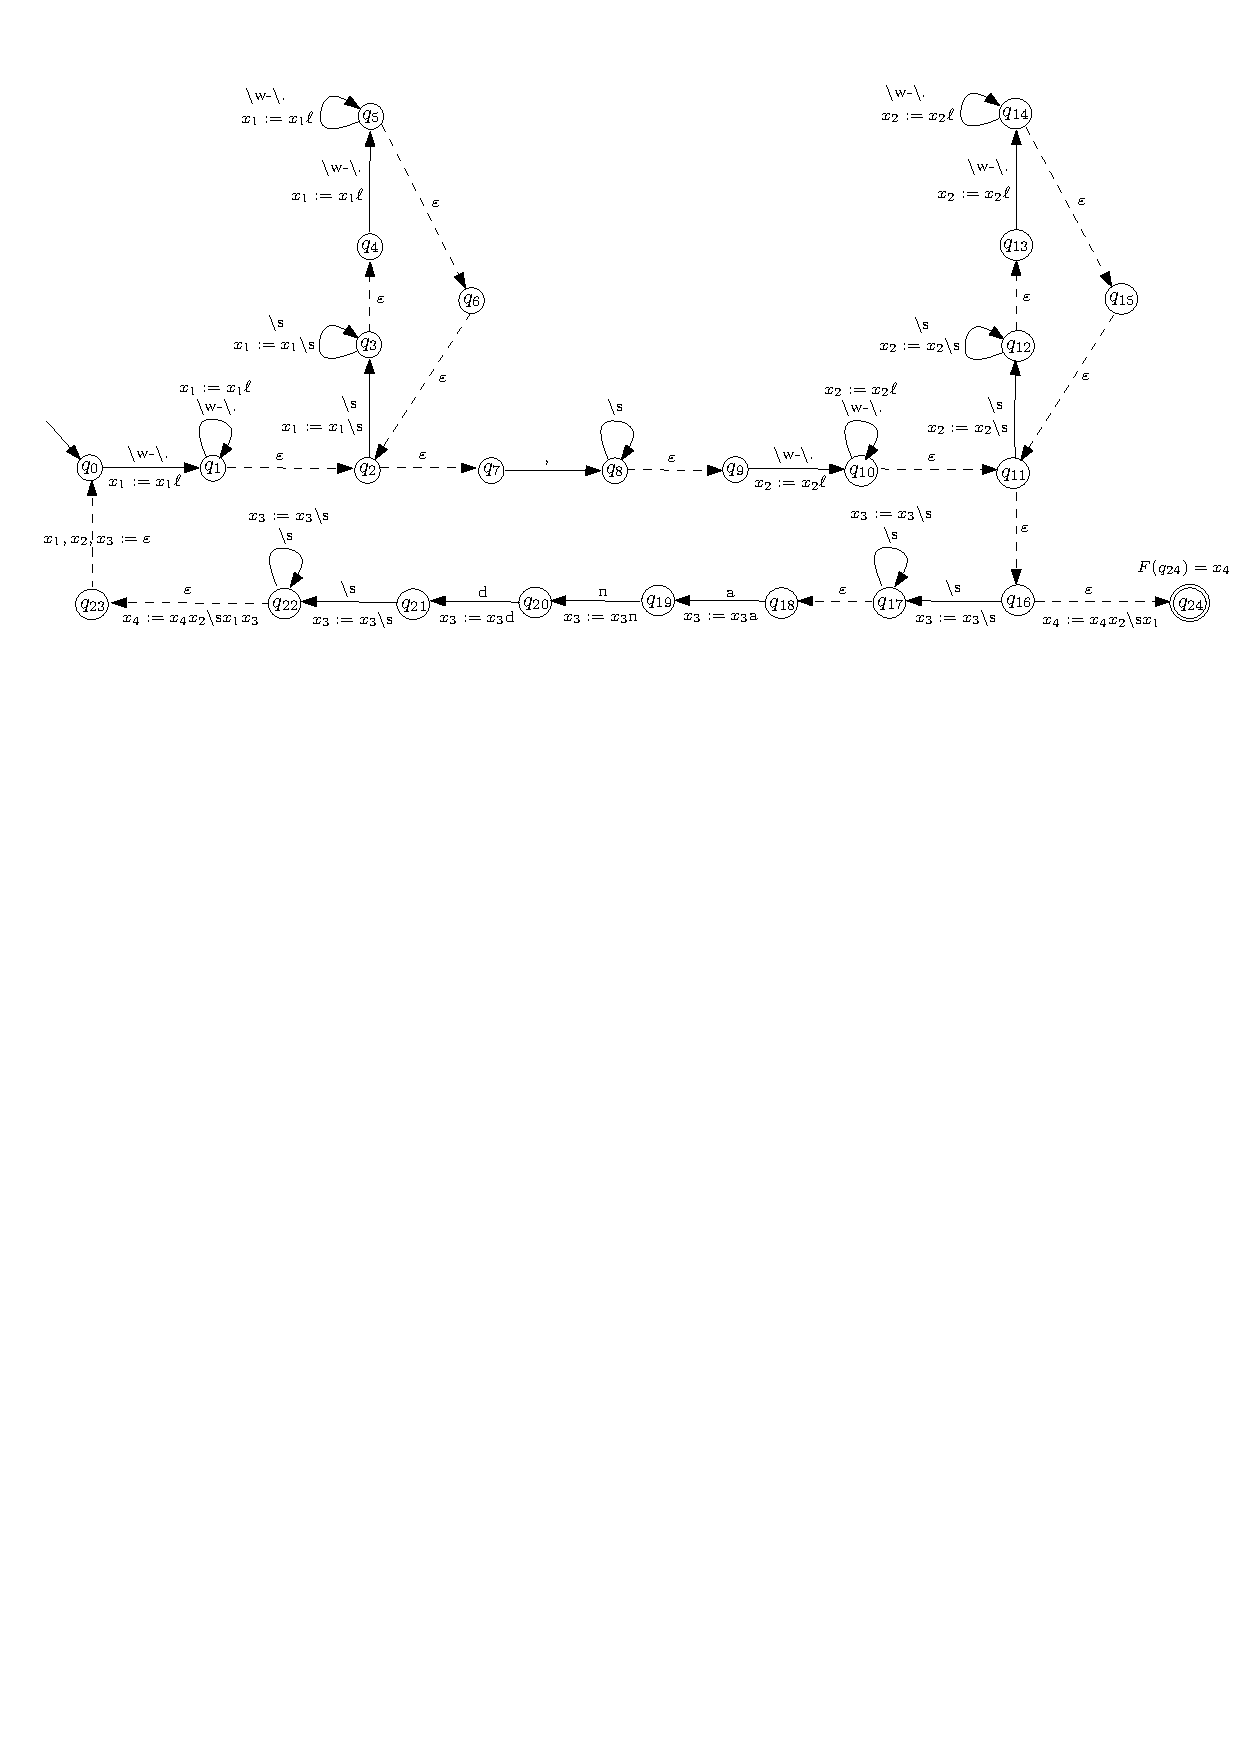
\includegraphics[scale=0.8]{psst-epsilon-exmp.pdf}
\caption{The PSST $\cT_{\sf nameReg}$}
\label{fig-psst-exmp}
\end{figure*}
\end{example}

  
%  $\tmop{Out} (r) =
%  s_{\varepsilon} \circ s_1 \circ s_2 \ldots s_n \circ F (q_n)$ where
%  $s_{\varepsilon}$ is the empty substitution which maps all variables to
%  $\varepsilon$.
  
\begin{definition}[Pre-image]
For a string relation $R \subseteq \Sigma^* \times \Sigma^*$ and $L \subseteq \Sigma^*$, we define the \emph{pre-image} of $L$ under $R$ as $R^{-1}(L):=\{w \in \Sigma^* \mid \exists w'.\ w' \in L \mbox{ and } (w, w') \in R\}$. 
\end{definition}
 
\begin{theorem}[Pre-image of \PSST{}]
  \label{theorem:psst_preimage}
  Given a \PSST{} $\psst = (Q_T, \Sigma$, $X, \delta_T, \tau_T, E_T,  q_{0, T}, F_T)$ and an \FA{} $\Aut
  = (Q_A, \Sigma, \delta_A, q_{0, A}, F_A)$, we can compute an \FA{} $\cB = (Q_B,
  \Sigma, \delta_B, q_{0, B}, F_B)$ in exponential time  such that $\Lang(\cB) = \cR^{-1}_{\cT}(\Lang(\Aut))$.
\end{theorem}
 
\begin{proof}
Without loss of generality, we assume that $\Aut$ contains no $\varepsilon$-transitions. 
Intuitively, $\cB$ simulates the run of $\psst$ on $w$, and, for each $x \in X$, records the set of state pairs $(p, q) \in Q_A \times Q_A$ such that starting from $p$, $\Aut$ can reach $q$ after reading the string stored in $x$. Moreover, $\cB$ also records all the states accessible from a run with higher priority to ensure the current run is the accepting one of $\psst$.

Before the formal construction of $\cB$, we introduce some notations.
\begin{itemize}
\item For $S \subseteq Q_T$, $\delta^{(ip)}_T(S, a) = \{q'_1 \mid \exists q_1 \in S, q'_1 \in \delta_T(q_1, a)\}$.
%
\item For $q \in Q_T$,  if $\tau_T(q) = (P_1, P_2)$, then $\tau^{(ip)}_T(\{q\})=S$ such that $S$ is the set of states occurring in $P_1$ and $P_2$. Moreover, for $S \subseteq Q_T$, we define $\tau^{(ip)}_T(S) = \bigcup \limits_{q \in S} \tau^{(ip)}_T(\{q\})$. 
%
We also use $(\tau^{(ip)}_T)^\ast$ to denote the reflexive transitive closure of $\tau^{(ip)}_T$.
%\item For $\sigma \in \Sigma$ and $S \subseteq Q_T$,  we use $\tau^+_T[a, S]$ to denote the set of states that can be obtained from 
% 
\item For $\rho \in (\cP(Q_A \times Q_A ))^{X}$ and $s \in X \rightarrow (X \cup \Sigma)^{\ast}$, we use $s(\rho)$ to denote $\rho'$ that is obtained from $\rho$ as follows: For each $x \in X$, if $s(x) = \varepsilon$, then $\rho'(x) = \{(p, p) \mid p \in Q_A\}$, otherwise, let $s(x) = b_1 \cdots b_\ell$ with $b_i \in \Sigma \cup X$ for each $i \in [\ell]$, then $\rho'(x) = \theta_1 \circ \cdots \circ \theta_\ell$, where $\theta_i = \delta^{(b_i)}_A$ if $b_i \in \Sigma$, and $\theta_i = \rho(b_i)$ otherwise.
\end{itemize}

We are ready to present the construction of $\cB =  (Q_B$, $\Sigma$, $\delta_B$, $q_{0, B}, F_B)$: $Q_B = Q_T \times (\cP(Q_A \times Q_A ))^{X} \times \cP(Q_T)  $, $q_{0, B} = (q_{0, T}, \rho_{\varepsilon}, \emptyset)$ where $\rho_{\varepsilon} (x) = \{(q, q) \mid q \in Q\}$ for each $x \in X$, and $\delta_{B}$ comprises 
\begin{itemize}
\item the tuples $((q, \rho, S), \sigma, (q_i, \rho', S'))$ such that $\sigma \in \Sigma$ and there exists $s \in \left((X \cup \Sigma\right)^*)^X$ satisfying
\begin{itemize}
\item $\delta_T (q, \sigma) = (q_1, \ldots, q_i, \ldots, q_m)$, 
%
\item $s = E(q, \sigma, q_i)$,
%
\item let $\tau^{(ip)}(q) = (S_1, S_2)$ and $(\tau^{(ip)}_T)^\ast(S \cup S_1) = S''$, then $S' =  \delta^{(ip)}_T(S'', \sigma)$ $\cup$ $\{ q_1$, $\ldots$, $q_{i - 1} \}$, 
\item $\rho' = s(\rho)$;
%
%$\rho'(x) = \theta_\ell$ such that $\theta_0 = \{(p,p) \mid p \in Q_A\}$, and for each $i \in [\ell]$, if $b_i \in \Sigma$, then $\theta_i = \{(p, p') \mid (p, p'') \in \theta_{i-1}, (p'', b_i, p') \in \delta_A \mbox{ for some } p''\}$, otherwise, $\theta_i = \theta_{i-1} \cdot \rho(x)$. 
\end{itemize}
%
\item the tuples $((q, \rho, S), \varepsilon, (q_i, \rho', S'))$ such that there exists $s \in \left((X \cup \Sigma\right)^*)^X$ satisfying
\begin{itemize}
\item $\tau_T (q) = ((q_1, \ldots, q_i, \ldots, q_m); \cdots)$, 
%
\item $s = E(q, \varepsilon, q_i)$,
%
\item $S' =  \tau^{(ip)}_T(S) \cup   \{ q_1, \ldots, q_{i - 1} \}$, 
\item $\rho' = s(\rho)$;
%
%$\rho'(x) = \theta_\ell$ such that $\theta_0 = \{(p,p) \mid p \in Q_A\}$, and for each $i \in [\ell]$, if $b_i \in \Sigma$, then $\theta_i = \{(p, p') \mid (p, p'') \in \theta_{i-1}, (p'', b_i, p') \in \delta_A \mbox{ for some } p''\}$, otherwise, $\theta_i = \theta_{i-1} \cdot \rho(x)$. 
\end{itemize}
%
\item the tuples $((q, \rho, S), \varepsilon, (q_i, \rho', S'))$ such that there exists $s \in \left((X \cup \Sigma\right)^*)^X$ satisfying
\begin{itemize}
\item $\tau_T (q) = ((q'_1, \ldots, q'_n); (q_1, \ldots, q_i, \ldots, q_m))$, 
%
\item $s = E(q, \varepsilon, q_i)$,
%
\item $S' =\tau^{(ip)}_T(S) \cup  \{q'_1, \ldots, q'_n, q_1, \ldots, q_{i - 1} \}$, 
\item $\rho' = s(\rho)$.
%
%$\rho'(x) = \theta_\ell$ such that $\theta_0 = \{(p,p) \mid p \in Q_A\}$, and for each $i \in [\ell]$, if $b_i \in \Sigma$, then $\theta_i = \{(p, p') \mid (p, p'') \in \theta_{i-1}, (p'', b_i, p') \in \delta_A \mbox{ for some } p''\}$, otherwise, $\theta_i = \theta_{i-1} \cdot \rho(x)$. 
\end{itemize}
\end{itemize}

Moreover, $F_B$ is the set of states $(q, \rho, S) \in Q_B$ such that
\begin{enumerate}
  \item $F_T (q)$ is defined,
%
  \item for any $q' \in S$, $F_T (q')$ is not defined,
  %
  \item if $F_T(q) = \varepsilon$, then $q_{0, A}  \in F_A$, otherwise, 
let $F_T(q) = b_1 \cdots b_\ell$ with $b_i \in \Sigma \cup X$ for each $i \in [\ell]$, then $(\theta_1 \circ \cdots \circ \theta_\ell) \cap (\{q_{0,A}\} \times F_A) \neq \emptyset$, where for each $i \in [\ell]$, if $b_i \in \Sigma$, then $\theta_i = \delta^{(b_i)}_A$, otherwise, $\theta_i = \rho(b_i)$.
\end{enumerate}
\end{proof}

Note that the above construction  does not utilize the so-called \tmtextit{copyless} property \cite{AC10,AD11},
  thus it works for general, or \tmtextit{copyful} \PSST{} \cite{FR17}.

% Note that in the definition of \NSST, there is no \emph{copyless} restriction.



